\documentclass[border=2pt]{standalone}

% Drawing
\usepackage{tikz}

% Circuits
\usepackage{circuitikz}
%% Specifications
\ctikzset{bipoles/thickness=1.2}

% Styles
\tikzset{>=latex}

% Tikz Library
\usetikzlibrary{angles,quotes}

% Define Color
\definecolor{bleudefrance}{rgb}{0.19, 0.55, 0.91}

% Notation
\usepackage{amsmath}
\usepackage{siunitx}

\begin{document}
	
	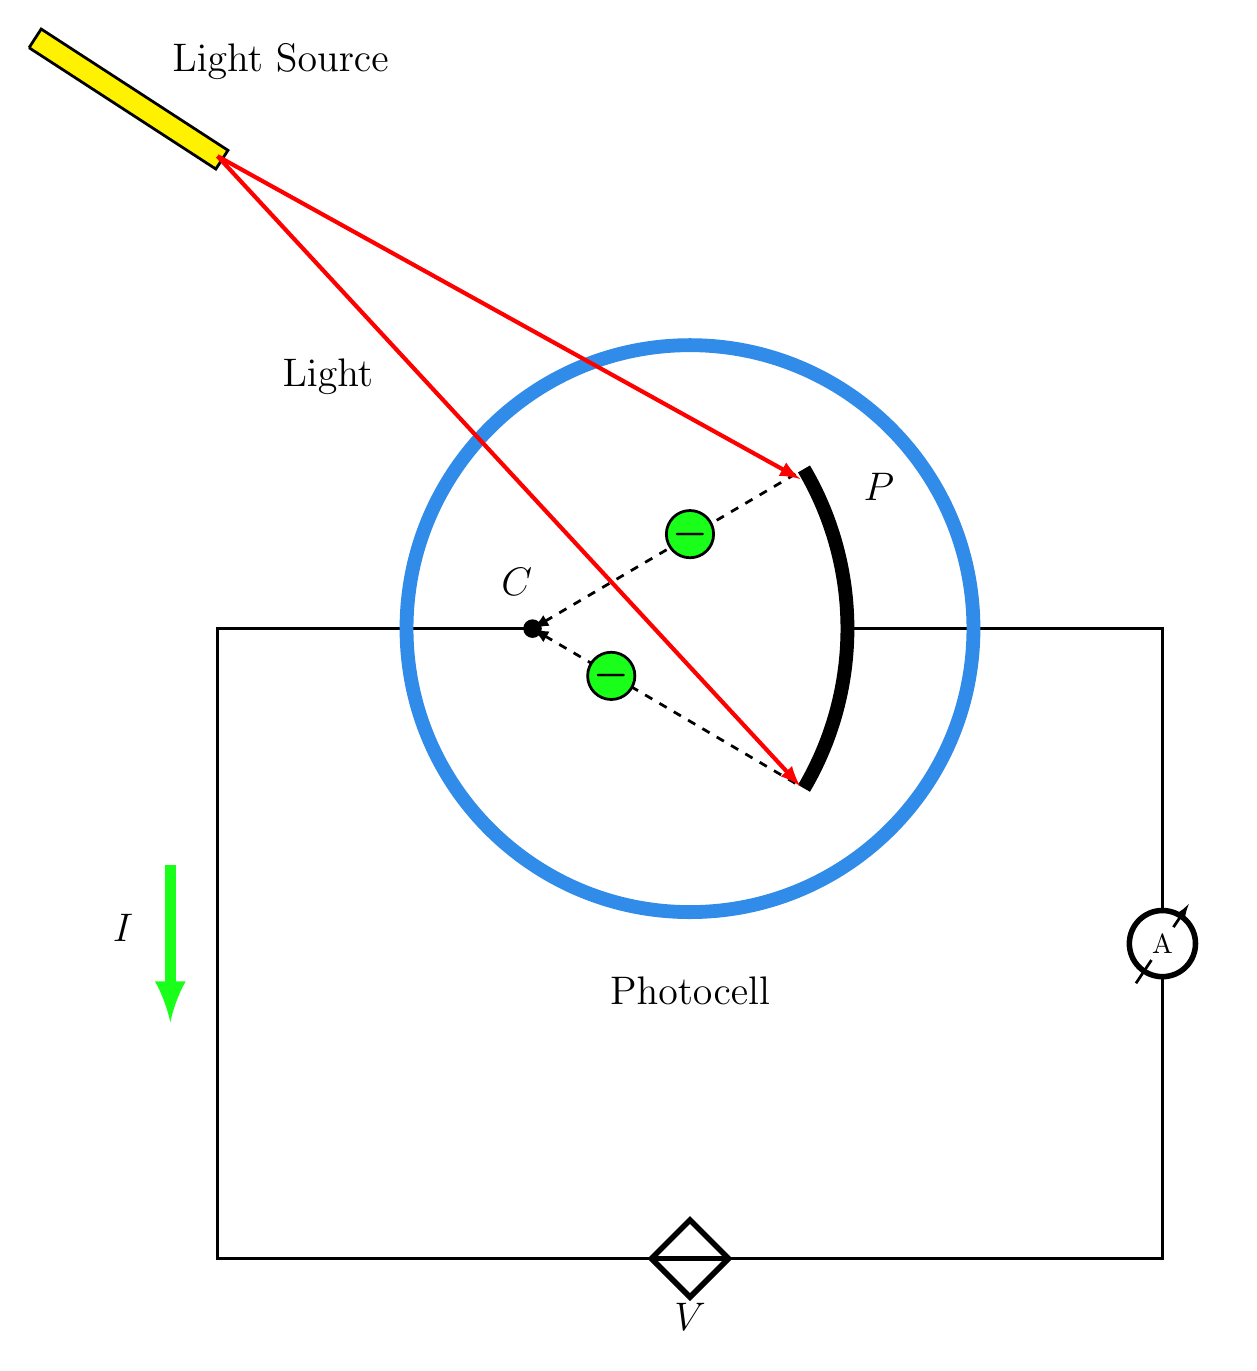
\begin{tikzpicture}[scale=2, line width=1]
		% Grid
%		\draw[help lines] (0,0) grid (11,11);
		
		% Circuits		
		\draw (4,6) -- (2,6) -- (2,2) to[controlled voltage source, l_=\Large$V$] ++(6,0) to[rmeterwa, t=$\si{A}$] ++(0,4) -- +(-2,0);
		\filldraw (4,6) circle [radius=0.05];
		
		% Dashed Arrows
		\draw[dashed,<-] (4,6) -- +(1.7,1)coordinate(A);
		\draw[dashed,<-] (4,6)coordinate(B) -- +(1.7,-1)coordinate(C);
		
		% Arc		
		\pic [draw, angle radius= 4 cm, line width = 5] {angle=C--B--A};
		
		% Photocell
		\draw[color=bleudefrance, line width=5] (5,6) circle [radius=1.8];
		
		% Laser
		\draw[fill=yellow, line width=1, rotate=12] (2.8,9.31) -- ++(1,-1) -- ++(0.1,0.1) -- ++(-1,1) -- +(-0.1,-0.1);
		%% Rays
		\draw[line width=1.5, red, <-] (5.7,5) -- (2,9);
		\draw[line width=1.5, red, <-] (5.7,6.95) -- (2,9);
		
		% Electrons		
		\draw[fill=green!90] (4.5,5.7) circle [radius = 0.15];
		\draw[fill=green!90] (5,6.6) circle [radius = 0.15];
		%% Minus Symbol
		\node at (5,6.6) {\Large $\boldsymbol{-}$};
		\node at (4.5,5.7) {\Large$\boldsymbol{-}$};
		
		% Current (Green Arrow)
		\draw[green!90, ->, line width = 4] (1.7,4.5) -- +(0,-1);
		
		% Nodes
		\node at (1.4,4.1) {\Large$I$};
		\node at (3.9,6.3) {\Large $C$};
		\node at (6.2,6.9) {\Large$P$};
		\node at (2.4,9.6) {\Large Light Source};
		\node at (2.7,7.6) {\Large Light};
		\node at (5,3.7) {\Large Photocell};
	\end{tikzpicture}
	
\end{document}